\documentclass[9pt,colorlinks]{beamer}
  % compress
  %\documentclass[handout,xcolot=pdftex,dvipsnames,table]{beamer}
\definecolor{mybg}{RGB}{255,255,204}

\usepackage[english]{babel}
\usepackage[utf8x]{inputenc}

\usepackage{xcolor}
%\usepackage[colorlinks = true,
%            linkcolor = blue,
%            urlcolor  = blue,
%            citecolor = blue,
%            anchorcolor = blue]{hyperref}
%\usepackage{amsmath}


\usepackage{graphicx}
 % \usepackage{beamerthemesplit}

%\usemintedstyle{trac}

\mode<presentation>
\setbeamercovered{invisible}
\usetheme{Warsaw}
\usecolortheme{dolphin}

\usefonttheme{serif}










\title{ Python in a Nutshell}
\subtitle
 {Introdution } % (optional)


\author[Velasco and Perera]{Manel Velasco,\inst{1} PhD and Alexandre Perera,\inst{1}$^{,}$\inst{2} PhD}

\institute[UPC] % (optional, but mostly needed)
{
  \inst{1}%
  Departament d'Enginyeria de Sistemes, Automatica i Informatica Industrial (ESAII)  \\
  Universitat Politecnica de Catalunya 
  \and 
  \inst{2}%
   Centro de Investigacion Biomedica en Red en Bioingenieria, Biomateriales y Nanomedicina (CIBER-BBN)  \\
    \href{mailto:Alexandre.Perera@upc.edu}{Alexandre.Perera@upc.edu}~\href{mailto:manel.velasco@upc.edu}{Manel.Velasco@upc.edu}
}
 

\date[Feb, 2013, Learning Python]{Introduction to Python for Engineering and Statistics\\
Febraury, 2013}

 %

\begin{document}


\begin{frame}[plain]
   %  \titlepage
   \maketitle
\end{frame}


\section{Content}


\begin{frame}
	\setbeamercovered{dynamic}
	\frametitle{ Course outline}
The course is structure on four parts:
\begin{enumerate}
    \item Python: language, structure, mutable/inmutable objects, functions.
     \item Numpy and plotting (Matplotlib and Mayavi)
     \item Scipy. Simpy.
     \item Scikits. Machine learning with Scikit-learn. An eigenfaces session with scikit-learn 
\end{enumerate}

\end{frame}
\section{Authors} % (fold)
\label{sec:Authors}

% section Authors (end)
%----------------------------FRAME 2 cols------------------------------
\begin{frame}[shrink]\frametitle{Scipy Lecture Notes}
    \small Some parts of this seminar contains text and material from \href{http://scipy-lectures.github.com/}{http://scipy-lectures.github.com's Scipy Lecture Notes}. This is an open-source python course project for creating teaching material on the scientific Python ecosystem, central tools and techniques.

    \Tiny
\begin{columns}[c]
\column{0.5\textwidth}
\begin{block}{Editors}
\begin{itemize}
    \item Valentin Haenel
    \item Emmanuelle Gouillart
    \item  Gaël Varoquaux
\end{itemize}          
\end{block}
\begin{block}{Additional Contributors}

    \begin{itemize}  
        \item  Akihiro Uchida
        \item Corey Farwell
        \item egens
        \item Lars Buitinck
        \item  Olivier Verdier
        \item Virgile Fritsch
    \end{itemize}
\end{block}

\column{0.5\textwidth}
\begin{block}{Authors}
\begin{itemize}
    \item  Christopher Burns
    \item Adrian Chauve
    \item Robert Cimrman
    \item Christophe Combelles
    \item André Espaze
    \item Emmanuelle Gouillart
    \item Mike Müller
    \item Fabian Pedregosa
    \item Didrik Pinte
    \item Nicolas Rougier
    \item Gaël Varoquaux
    \item Pauli Virtanen
    \item Zbigniew Jedrzejewski-Szmek
\end{itemize}
\end{block}
\end{columns}

\end{frame}


%----------------------------FRAME 2 cols + header (box)-------------
\begin{frame}[plain]\frametitle{About Us}
\begin{block}{Manel Velasco, PhD}
    \small Manel Velasco graduated in maritime engineering in 1999 and received the PhD degree in automatic control in 2006, both from the Technical University of Catalonia, Barcelona, Spain.  He has been involved in research on artificial intelligence from 1999 to 2002 and, since 2000, on the impact of real-time systems on control systems. His research interests include artificial intelligence, real-time control systems, and collaborative control systems, especially on redundant controllers and multiple controllers with self-interacting systems.
\end{block}

    \begin{columns}[c]
\column{0.65\textwidth}

Automatic Control Department\\
Universitat Politècnica de Catalunya\\
Pau Gargallo, 5\\
08028 Barcelona (Spain)\\
Phone: +34 93 401 1681\\
Fax: +34 93 401 7045\\
\href{manel.velasco@upc.edu}{manel.velasco@upc.edu}
\column{0.35\textwidth}
\begin{figure}[!htb]
    \centering
    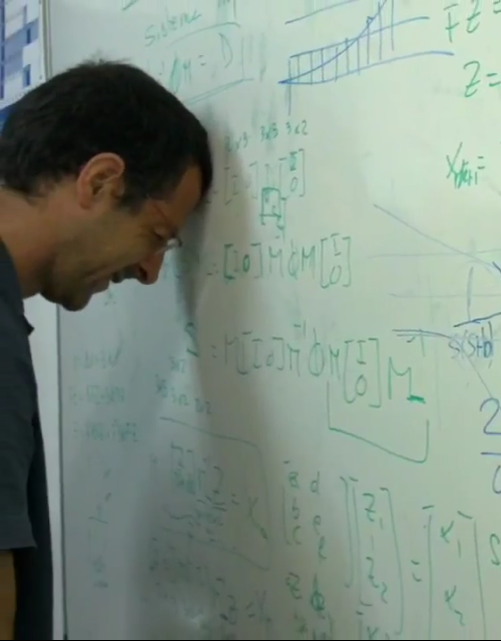
\includegraphics[width=\textwidth]{figs/manel}
\end{figure}
\end{columns}
\end{frame}

%----------------------------FRAME 2 cols + header (box)-------------
\begin{frame}[plain]\frametitle{About Us}

\begin{block}{Alexandre Perera, PhD}

    \small Alexandre Perera-LLuna graduated in physics at University of Barcelona at 1999 and in electrical engineering at 2001, he received a PhD degree in physics from the same university in 2003. He stayed as a postdoctoral fellow at Texas A\&M University (USA) and in Universitat Politècnica de Catalunya(Spain) as a Ramon y Cajal Fellow from 2008-1012. His main area of expertise covers machine learning, statistical analysis, and data mining in biomedical systems, bioengineering and bioinformatics. He is an Associate Professor at Universitat Politècnica de Catalunya-BarcelonaTech (UPC).
\end{block}
\begin{columns}[c]
\column{0.65\textwidth}
Automatic Control Department\\
Universitat Politècnica de Catalunya\\
Pau Gargallo, 5\\
08028 Barcelona (Spain)\\
Phone: +34 93 401 6963\\
Fax: +34 93 401 7045\\
\href{Alexandre.Perera@upc.edu}{Alexandre.Perera@upc.edu}

 
\column{0.35\textwidth}
\begin{figure}[!htb]
    \centering
    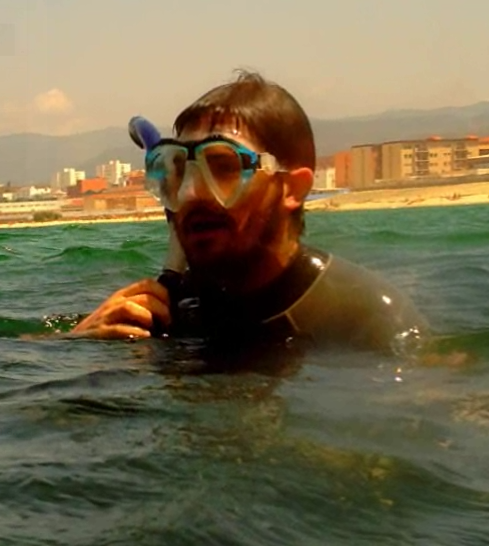
\includegraphics[width=\textwidth]{figs/alex1}
\end{figure}
\end{columns}
\end{frame}
\section{Preparation} % (fold)
\label{sec:Preparation}

% section Preparation (end)
%----------------------------FRAME------------------------------------
\begin{frame}[fragile]\frametitle{About this course}
\begin{block}{}


    \begin{itemize}
        \item All material has been prepared with \LaTeX~ and edited on \href{http://www.vim.org}{Vim} by disgrace of Alex (an emacs guy).
        \item Python snippets have been embedded into \LaTeX with help of \href{http://mpastell.com/pweave/}{Pweave}, developed by Matti Pastell. 
        \item All Python code and results has been highlighted through \emph{minted} package, developed by Konrad Rudolph, the \emph{python syntax highlighter} \href{http://pygments.org}{Pygments}, and custom build bash hacks because the world is not really perfect. 

    \end{itemize}
    \end{block}

\end{frame}


\begin{frame}\frametitle{For practical sessions}
\begin{figure}[!htb]
    \centering
    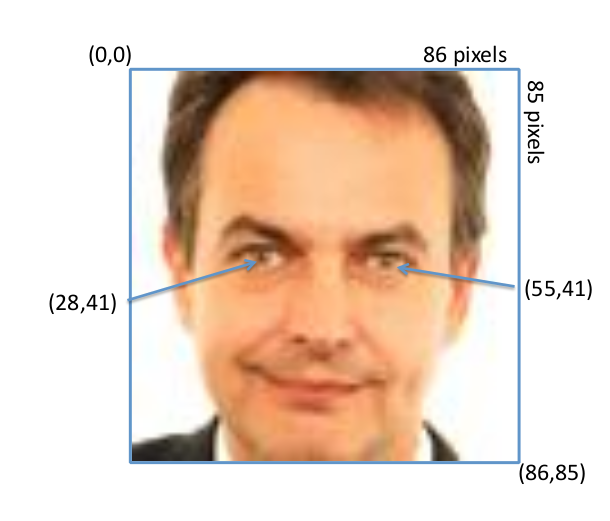
\includegraphics[width=0.7\textwidth]{figs/format}
\end{figure}
\end{frame}


%----------------------------FRAME------------------------------------
\begin{frame}\frametitle{Let's start!}
\begin{figure}[!htb]
    \centering
    
\includegraphics[width=0.6\textwidth]{figs/question}
\end{figure}
\end{frame}


\end{document}
